\section{Examination of Numerical Accuracy}


%%%%%%%%%%%%%%%%%%%%%%%%%%%%%%%%%%%%%%%%%%%%%%%
%%%%%%%%%%%%%%%%%%%%%%%%%%%%%%%%%%%%%%%%%%%%%%%
\FloatBarrier
\subsection{Uniaxial Compression with Finite Rotation}
%
For the sake of comparison with the strongly objective algorithm proposed in \cite{rashid1993}, an example problem similar to the one given therein will be considered, consisting of a block of isotropic material which is compressed uniaxially and simultaneously rotated according to the deformation gradient given by
\begin{equation}
    \mathbf{F} = \mathbf{R} \mathbf{U} = \left[ \begin{array}{ccc} \cos \omega t & - \sin \omega t & 0 \\ \sin \omega t & \cos \omega t & 0 \\ 0 & 0 & 1 \end{array} \right] \left[ \begin{array}{ccc} 1 - \beta t & 0 & 0 \\ 0 & 1 & 0 \\ 0 & 0 & 1 \end{array} \right],
\end{equation}
The material model will be chosen as the isotropic hypoelastic model of grade zero, i.e.
\begin{equation}
    \overset{\circ}{\mathbf{T}} = \lambda \mathbf{1} \text{tr} (\mathbf{D}) + 2 \mu \mathbf{D},
\end{equation}
where $\lambda = E \nu / (1+\nu)(1-2\nu)$ and $\mu = E/2(1+\nu)$ are the standard Lam\'{e} parameters. Exact solutions for the Cauchy stress components according to the Jaumann rate are easily obtained for this problem:
\begin{equation}
  \left\{ \begin{array}{c} T_{11} \\ T_{22} \\ T_{33} \\ T_{23} \\ T_{13} \\ T_{12} \end{array} \right\} = \left\{ \begin{array}{c} \left[ \lambda + \mu (1 - \cos 2 \omega t) \right] \ln (1 - \beta t) \\ \left[ \lambda + \mu (1 + \cos 2 \omega t) \right] \ln (1-\beta t) \\ \lambda \ln (1-\beta t) \\ 0 \\ 0 \\ -\mu (\sin 2 \omega t) \ln (1-\beta t) \end{array} \right\}.
\end{equation}
Numerical solutions were computed for the values $\omega = \pi$, $\beta = 0.5$, $E = 2.09 \times 10^5$, $\nu = 0.3$, and $t \in \left[ 0, 1 \right]$. The results are depicted in figure \ref{fig.v1-cm1}.

\begin{figure}
\centering
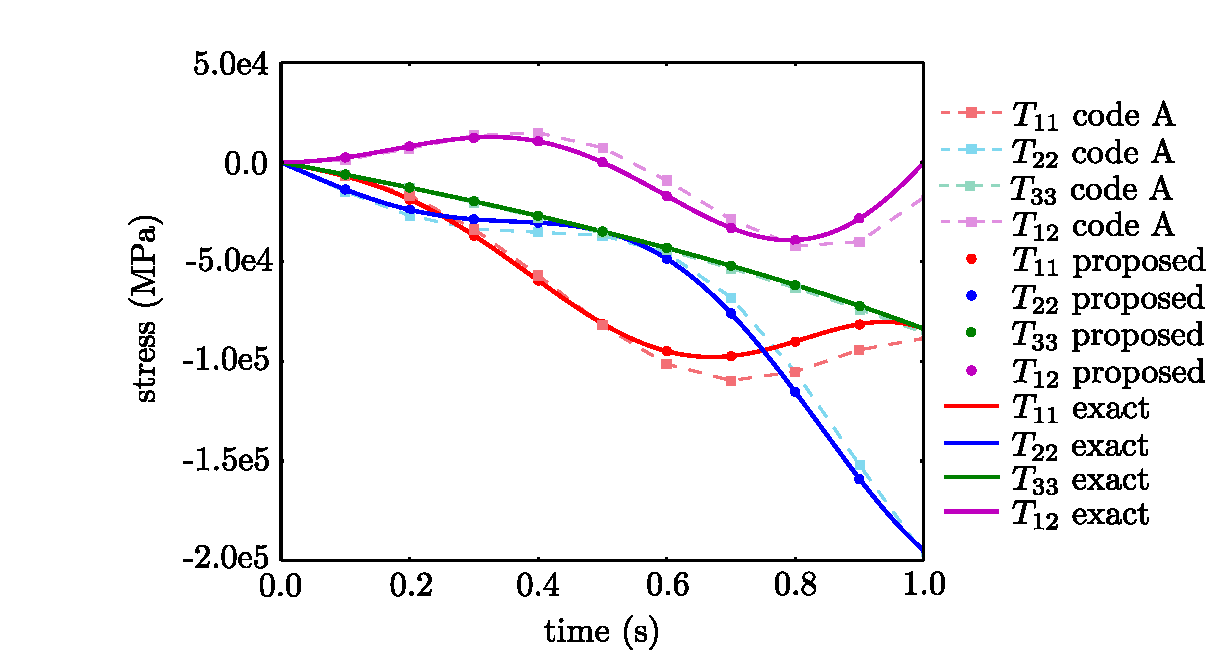
\includegraphics[scale=0.75]{media/stretch_rotate.pdf}
% where an .eps filename suffix will be assumed under latex,
% and a .pdf suffix will be assumed for pdflatex
\caption{Stress components plotted vs. time for the problem of uniaxial compression with finite rotation.}
\label{fig.v1-cm1}
\end{figure}

Worst-case relative errors between the exact solution $\mathbf{T}$ and approximate solutions $\mathbf{T}^h$ were computed via
\begin{equation}
    \text{\% error } (\mathbf{T}^h) = \sqrt{\frac{\max_{t} (\mathbf{T}^h - \mathbf{T}) \colon (\mathbf{T}^h - \mathbf{T})}{\max_{t} \mathbf{T} \colon \mathbf{T}}} \times 100 \% ,
    \label{eq:relative_error}
\end{equation}
and tabulated in table \ref{tab.v1-cm1}.

\begin{table}[]
\centering
\caption{Relative errors for the problem of uniaxial compression with finite rotation}
\label{tab.v1-cm1}
\begin{tabular}{c|c|c|c}
& code A & Rashid (1993) & proposed algorithm  \\ \hline
\% error $(\mathbf{T}^h)$ & 11.21704 & 0.01718 & 0.00014
\end{tabular}
\end{table}

%%%%%%%%%%%%%%%%%%%%%%%%%%%%%%%%%%%%%%%%%%%%%%%
%%%%%%%%%%%%%%%%%%%%%%%%%%%%%%%%%%%%%%%%%%%%%%%
\FloatBarrier
\subsection{Cyclic Shear}
%
In a retrospective examination of solution accuracy, the problem discussed in \cite{rashid1996} will be examined within the present context. The problem consists of a block of material which is subjected to a simple, cyclic shearing deformation given by
\begin{equation}
    \mathbf{F} = \left[ \begin{array}{ccc} 1 & \gamma & 0 \\ 0 & 1 & 0 \\ 0 & 0 & 1 \end{array} \right], \qquad \mathbf{L} = \left[ \begin{array}{ccc} 0 & \dot{\gamma} & 0 \\ 0 & 0 & 0 \\ 0 & 0 & 0 \end{array} \right],
\end{equation}
and where
\begin{equation}
    \gamma (t) = 2 \Gamma \bigg( \frac{2t}{T} - \left\lfloor \frac{2t}{T} + \frac{1}{2} \right\rfloor \bigg) (-1)^{\left\lfloor \frac{2t}{T} + \frac{1}{2} \right\rfloor}
\end{equation}
corresponds to the triangle wave with period $T$ and peak amplitude $\Gamma$, whose time derivative
\begin{equation}
    \dot{\gamma} (t) = \frac{4 \Gamma}{T} (-1)^{\left\lfloor \frac{2t}{T} + \frac{1}{2} \right\rfloor}
\end{equation}
is the square wave with period $T$. As before, the isotropic hypoelastic model of grade zero will be employed, where $\mu = E/2(1+\nu)$ represents the shear modulus of the material. The exact solution for the Cauchy stress components according to the Jaumann rate is given by the solution to the differential equation:
\begin{equation}
    \left\{ \begin{array}{c} \dot{T}_{11} \\ \dot{T}_{22} \\ \dot{T}_{12} \end{array} \right\} = \left[ \begin{array}{ccc} 0 & 0 & \dot{\gamma} \\ 0 & 0 & - \dot{\gamma} \\ -\dot{\gamma}/2 & \dot{\gamma}/2 & 0 \end{array} \right] \left\{ \begin{array}{c} T_{11} \\ T_{22} \\ T_{12} \end{array} \right\} + \mu \left\{ \begin{array}{c} 0 \\ 0 \\ \dot{\gamma} \end{array} \right\},
\end{equation}
which yields
\begin{equation}
    \left\{ \begin{array}{c} T_{11} \\ T_{22} \\ T_{33} \\ T_{23} \\ T_{13} \\ T_{12} \end{array} \right\} = \left\{ \begin{array}{c} \mu (1-\cos \gamma (t)) \\ \mu (\cos \gamma (t) - 1) \\ 0 \\ 0 \\ 0 \\ \mu \sin \gamma (t) \end{array} \right\}.
\end{equation}
Numerical solutions were computed for the values $\Gamma = 0.5$, $E = 2.09 \times 10^5$, $\nu = 0.3$, $T = 1.0$, and $t \in \left[ 0, 2 \right]$, yielding 2 complete cycles of deformation. The results are depicted in figure \ref{fig.cyclic_shear-cm1}.

\begin{figure}
\centering
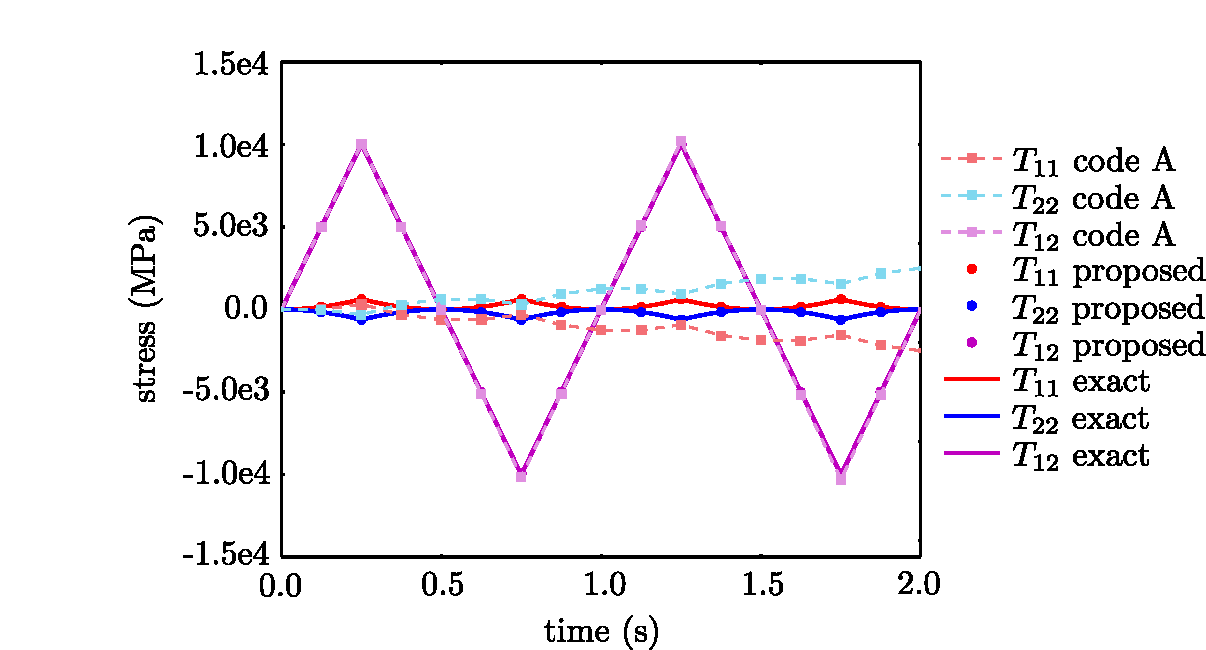
\includegraphics[scale=0.75]{media/cyclic_shear.pdf}
% where an .eps filename suffix will be assumed under latex,
% and a .pdf suffix will be assumed for pdflatex
\caption{Stress components plotted vs. time for the problem of cyclic shear.}
\label{fig.cyclic_shear-cm1}
\end{figure}

Worst-case relative errors between the exact solution $\mathbf{T}$ and approximate solutions $\mathbf{T}^h$ were computed via equation \ref{eq:relative_error} and tabulated in table \ref{tab.cyclic_shear-cm1}.

\begin{table}[]
\centering
\caption{Relative errors for the problem of cyclic shear}
\label{tab.cyclic_shear-cm1}
\begin{tabular}{c|c|c|c}
& code A & Rashid (1993) & proposed algorithm  \\ \hline
\% error $(\mathbf{T}^h)$ & 24.94638 & 0.00227 & 0.00205
\end{tabular}
\end{table}

%%%%%%%%%%%%%%%%%%%%%%%%%%%%%%%%%%%%%%%%%%%%%%%
%%%%%%%%%%%%%%%%%%%%%%%%%%%%%%%%%%%%%%%%%%%%%%%
\FloatBarrier
\subsection{Twisting Prism}

\begin{figure}[!tbhp]
\centering
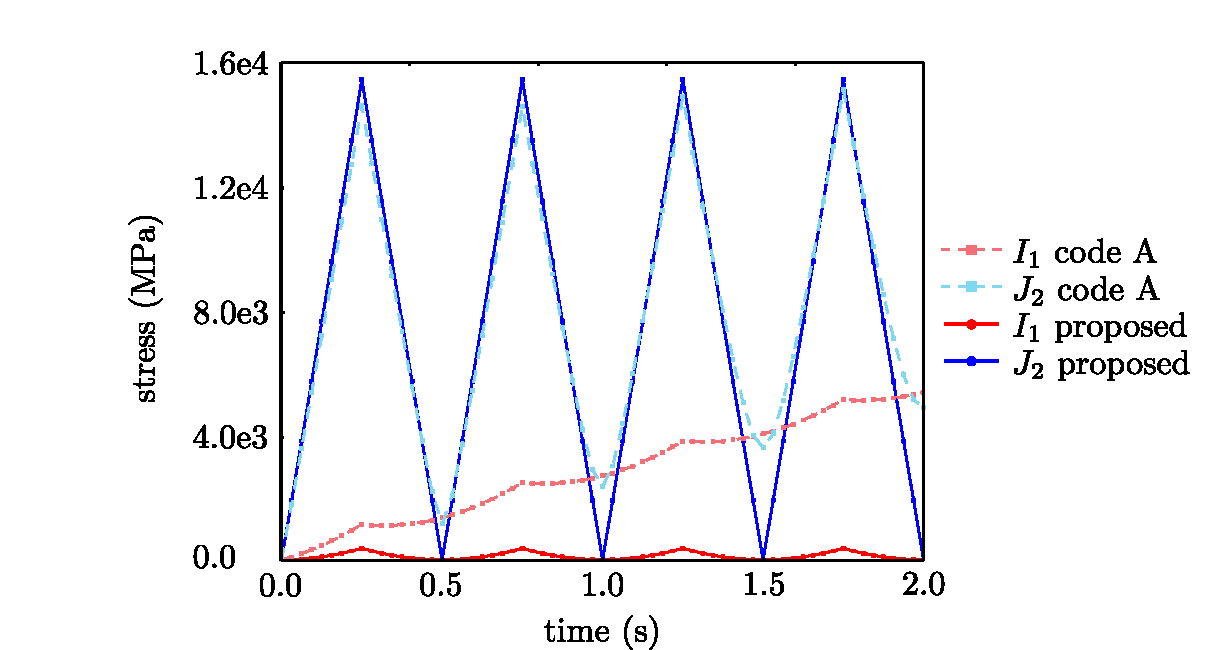
\includegraphics[scale=0.75]{media/twisted_prism.pdf}
% where an .eps filename suffix will be assumed under latex,
% and a .pdf suffix will be assumed for pdflatex
\caption{Stress measures plotted vs. time for the twisting prism problem, where $I_1$ is the first invariant of the Cauchy stress tensor, and $J_2$ is the second invariant of the deviatoric stress tensor}
\label{fig.twisted_prism-cm1}
\end{figure}
\negparafig

%%%%%%%%%%%%%%%%%%%%%%%%%%%%%%%%%%%%%%%%%%%%%%%
%%%%%%%%%%%%%%%%%%%%%%%%%%%%%%%%%%%%%%%%%%%%%%%